	\documentclass[10pt,oneside]{CBFT_book}
	% Algunos paquetes
	\usepackage{amssymb}
	\usepackage{amsmath}
	\usepackage{graphicx}
% 	\usepackage{libertine}
% 	\usepackage[bold-style=TeX]{unicode-math}
	\usepackage{lipsum}

	\usepackage{natbib}
	\setcitestyle{square}

	\usepackage{polyglossia}
	\setdefaultlanguage{spanish}
	



	\usepackage{CBFT.estilo} % Cargo la hoja de estilo

	% Tipografías
	% \setromanfont[Mapping=tex-text]{Linux Libertine O}
	% \setsansfont[Mapping=tex-text]{DejaVu Sans}
	% \setmonofont[Mapping=tex-text]{DejaVu Sans Mono}

	%===================================================================
	%	DOCUMENTO PROPIAMENTE DICHO
	%===================================================================

\begin{document}

% =================================================================================================
\chapter{Introducción al estudio de procesos de relajación}
% =================================================================================================


% =================================================================================================
\section{Procesos de Markov}
% =================================================================================================

Sea $Y$ una variable estocástica (aquellas que provienen de experimentos, donde no se tiene información
dinámica determinista\footnote{No tengo información para predecir nada.}) 
que puede tomar valores $y_1, y_2,...$\notamargen{Las $P$ son densidades
de probabilidad, cuando el espacio muestral sea continuo.}
\[
	P_1(y_1,t) \equiv \text{Prob. de tomar $y_1$ en $t$ (1 paso)}
\]
\[
	P_2(y_1,t_1;y_2,t_2) \equiv \text{Prob. conjunto de tomar $y_1$ en $t_1$ y $y_2$ en $t_2$}
\]
\[
	P_{1/1}(y_1,t_1 | y_2, t_2) \equiv \text{Prob. condicional de tomar $y_2$ en $t_2$ habiendo 
	tomado $y_1$ en $t_1$ (certeza de $y_1$) }
\]

Abreviaremos obviando el tiempo. Además se tiene 
\[
	P(y_1;y_2) \leq P(y_1 | y_2)
\]
donde el lhs evalúa los caminos que comunican $y_1, y_2$ del total y el rhs evalúa los cminos que comunican
$y_1, y_2$ del subconjunto de los que parten de $y_1$.

Además
\[
	P_2(y_1;y_2) = P_1(y_1) P_{1/1}(y_1|y_2)
\]
cumpliéndose lo siguiente
\begin{itemize}
 \item $ \int P_1(y_1) dy_1 = 1 \qquad  \text{normalización} $ 
 \item $ \int P_{1/1}(y_1|y_2) dy_2 = 1 \qquad \text{normalización} $ 
 \item $ \int P_2(y_1;y_2) dy_1 = \int P_1(y_1) P_{1/1}(y_1|y_2) dy_1 =  P_1(y_2) \qquad \text{reducción} $
\end{itemize}
La integral de normalización implica sumar todos los caminos de $(y_1,t_1)$ a $(y_2,t_2)$.

La reducción se puede definir en general para $N$ pasos y $N-1$.
Cuando la densidad de probabilidad es invariante ante una traslación temporal se dice que es estacionaria.

\subsubsection{Ejemplito numérico}

\[
	P(y_1;y_2) = P(y_1)P(y_1|y_2) = \frac{4}{4}\frac{1}{2} = \frac{2}{7}
\]
\[
	P(y_2;y_1) = P(y_2)P(y_2|y_1)  = \frac{3}{7}\frac{2}{3} = \frac{2}{7}
\]
Notemos que $P(A|B) \neq P(B|A)$ aunque $P(A;B) = P(B;A)$

Las densidades de muchos pasos: $P(y_1;y_2;y_3)$ son relevantes cuando el sistema tiene ``memoria''.
Se clasifican los procesos en función de la memoria; en el caso de Markov nos preocupamos del último
anerior y requeriré la probabilidad de un evento y la probabilidad de transición: estas dos cosas
definen los procesos de Markov.

Un proceso es de Markov cuando el estado del sistema depende del paso inmediato anterior únicamente.
Se define por 
\[
	P_1(y_1) , \quad P_{1/1}(y_1|y_2) \equiv \text{Probabilidad de transición} 
\]
\[
	P_{3/1}(y_1,y_2,y_3|y_4) \underbrace{\rightarrow}_{\text{Markov}} \; P_{1/1}(y_3|y_4)
\]

Se puede demostrar una ecuación de Chapman-Kolmogorov
\[
	P_{1/1}(y_1|y_3) = \int P_{1/1}(y_1|y_2) P_{1/1}(y_2|y_3) dy_2
\]
que se interpreta como la suma en todos los caminos. Se tiene el constraint de que la norma debe
conservarse en el tiempo.

% ~~~~~~~~~~~~~~~~~~~~~~~~~~~~~~~~~~~~~~~~~~~~~~~~~~~~~~~~~~~~~~~
\subsection{Ecuación maestra}

Queremos ver la evolución de la $P_1(y_1,t)$
\[
	\dtot{P_1(y,t)}{t} = \lim_{\tau \to 0} \frac{P_1(y,t+\tau) - P_1(y,t) }{\tau}
\]
Usando que
\[
	P_1(y_2,t+\tau) = \int dy_1 P_1(y_1,t) P_{1/1}(y_1,t|y_2,t+\tau) 
\]
\[
	P_1(y_2,t) = \int dy_1 P_1(y_1,t) P_{1/1}(y_1,t|y_2,t) 
\]
\[
	\dtot{P_1(y,t)}{t} = \int dy_1 P_1(y_1,t) \left[ \lim_{\tau \to 0} 
	\frac{1}{\tau} (P_{1/1}(y_1,t|y_2,t+\tau) - P_{1/1}(y_1,t|y_2,t))   \right]
\]
que se puede escribir de modo que 
\[
	\frac{1}{\tau} \left\{ [ 1 - \tau \int dy W(y_1,y)]\delta(y_1 - y_2) + 
	\tau W(y_1,y_2) - \delta(y_1-y_2) \right\}
\]
y entonces 
\[
	\dtot{P_1(y,t)}{t} = \int dy_1 P_1(y_1,t) 
	\left[ -\int dy W(y_1,y) \delta(y_1-y_2) + W(y_1,y_2) \right]
\]
\[
	\dtot{P_1(y,t)}{t} = \int dy_1 P_1(y_1,t) W(y_1,y_2) - \int dy_1 P_1(y_1,t) \int dy W(y_1,y)\delta(y_1-y_2)
\]
\[
	\dtot{P_1(y,t)}{t} = \int dy_1 P_1(y_1,t) W(y_1,y_2) - \int dy P_1(y_2,t) W(y_2,y)
\]
\[
	\dtot{P_1(y,t)}{t} = \int dy_1 P_1(y_1,t) W(y_1,y_2) - P_1(y_2,t) \int dy  W(y_2,y)
\]
donde el primer término en el rhs se interpreta como ganancia (lo que entra) y el segundo la
pérdida (pues la integral es lo que sale).
\[
	W(y_1,y_2) \equiv \text{Transiciones $y_1\to y_2$ por la unidad de tiempo}
\]

Si la densidad de probabilidad es nula puede ser que haya un balance entre lo IN y OUT.
Equilibrio no significa necesariamente que no pase nada; puede ser ese balance.


\begin{center}
	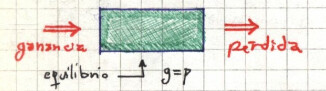
\includegraphics[scale=0.5]{images/1606329165.jpg}
	% asfdasdf.: 0x0 pixel, 0dpi, 0.00x0.00 cm, bb=
\end{center}


% ~~~~~~~~~~~~~~~~~~~~~~~~~~~~~~~~~~~~~~~~~~~~~~~~~~~~~~~~~~~~~~~
\subsection{Camino aleatorio y ecuación de difusión}

Si $\ell, \Tau$ son escalas y $n_2,s$ un número entero de pasos 
\[
	P_1(n_2\ell, s\Tau ) = 
	\sum_{n_1} P_1( n_1\ell, [s-1]\Tau )P_{1/1}( n_1\ell, [s-1]\Tau|n_2\ell, s\Tau )
\]
Quiero saber cuáles son las chances de estar en $n_2\ell$ al tiempo $s\Tau$ sumando todas 
las transiciones desde diferentes lugares $n_1\ell$.

Si la probabilidad es uniforme 
\[
	P_{1/1}(n_1\ell,[s-1]\Tau|n_2\ell,s\Tau) =
	\frac{1}{2}\delta(n_2-[n_1+1]) + \frac{1}{2}\delta(n_2-[n_1-1]) = \frac{1}{2}
	\begin{cases}
	 \text{si} \; n_2 = n_1 + 1 \\
	 \text{si} \; n_2 = n_1 - 1
	\end{cases}
\]
\[
	P_1(n_2\ell,s\Tau) = \sum_{n_1} P_1(n_1\ell,[s-1]\Tau)\left\{
	\frac{1}{2}\delta(n_2-[n_1+1]) + \frac{1}{2}\delta(n_2-[n_1-1])
	\right\}
\]
y sumando y restando convenientemente,
\[
	P_1(n_2\ell,s\Tau) = -\frac{1}{2}P_1([n_2-1]\ell,[s-1]\Tau) + 
\frac{1}{2}P_1([n_2+1]\ell,[s-1]\Tau)
	+ P_1(n_2\ell,[s-1]\Tau) - P_1(n_2\ell,[s-1]\Tau)
\]
\begin{multline}
	\frac{P_1(n_2\ell,s\Tau) - P_1(n_2\ell,s\Tau)}{\Tau} = \\
	\frac{\ell^2}{2\Tau} \left[ \frac{ P_1([n_2-1]\ell,[s-1]\Tau) - 
2P_1(n_2\ell,[s-1]\Tau) + P_1([n_2+1]\ell,[s-1]\Tau) }{\ell^2} \right] 
\end{multline}


Pero esto no es otra cosa que expresiones de las derivadas, de manera que
\[
	\frac{\delta P(n_2\ell,s\Tau)}{\delta \Tau} =
	\frac{\ell^2}{2\Tau} \frac{\delta^2 P(n_2\ell,[s-1]\Tau)}{\delta\ell^2}
\]

Esta es la ecuación de Fokker-Planck
\[
	\dpar{P(x,t)}{t} = C \dpar[2]{P(x,t)}{x}
\]
una ecuación de onda para la probabilidad (?)


\section{Cadenas de Markov}

Espacio muestral discreto $Y=\{ y_1, y_2, y_3,...,y_\ell \}$ de dimensión $L$ y donde
medimos el tiempo en pasos.
\[
	P_1(y_j,1) = \sum_i^L P_1(y_i,0) P_{1/1}(y_i,0|y_j,1)
\]
donde la información sobre las transiciones se introduce en
\[
	Q : Q_{ij} \equiv P_{1/1}(y_i,0|y_j,1)
\]
que es la matriz estocástica.
Se verifica
\[
	\sum_i^L Q_{ij} = 1 \; \forall i
\]
y entonces las filas son vectores de probabilidad\footnote{Tenía anotado que si
la suma de las filas es 1 entonces la matriz se llama estocástica}
\[
	\overbrace{\vec{P(1)}}^{1\times L} =  \overbrace{\vec{P(0)}}^{1\times L} 
\overbrace{Q}^{L\times L}
\]
\[
	P_j(1) = P_i(0) Q_{ij} \quad \text{Asumimos convención de Einstein}
\]
\[
	\vec{P(s)} = \vec{P(s-1)}Q = \vec{P(s-2)} Q Q = ... = \vec{P(0)}Q^s
\] 
y decimos que $Q$ es estocástica regular si existe $k : [Q^k]_{ij} > 0 \forall i,j$.

\notamargen{La matriz $Q$ tiene probabilidades de transición fijas en el tiempo,
de modo que $Q$ es independiente del tiempo.}

Si $Q$ es estocástica regular entonces existe $s : Q^{s+1} = Q^s \equiv T$ y por lo tanto
\[
	Q T = Q^{s+1} = T
\]
\notamargen{$T$ es la solución de equilibrio, pues $T=QT$}
Si $n>s$
\[
	\vec{P(n)} = \vec{P(0)} Q^n = \vec{P(0)} Q^{n-s} Q^s = \vec{P(0)} T
\]

\[
	\lambda_\alpha \overbrace{\vec{P}^\alpha}^{1\times L} =  
	\overbrace{\vec{P}^\alpha}^{1\times L} \overbrace{Q}^{L\times L}
	\quad \rightarrow \quad 0 = \vec{P}^\alpha (Q-\lambda_\alpha \mathbb{1}) 
\]
\[
	\lambda_\beta \overbrace{\vec{P}^\beta}^{1\times L} = 
	\overbrace{\vec{P}^\beta}^{1\times L} \overbrace{Q}^{L\times L}
	\quad \rightarrow \quad  0 = (Q-\lambda_\beta \mathbb{1}) \vec{P}^\beta
\]
\[
	\lambda_\alpha \chi_j^\alpha = \chi_{1i}^\alpha Q_{ij} \qquad \vec{\chi} = (,,,)
\]
donde los índices $j,1i$ refieren a columnas y
\[
	\lambda_\beta \psi_{i1}^\beta = Q_{ij} \psi_{j1}^\beta \qquad \vec{\chi} = 
\begin{pmatrix}
                                                                            \\
                                                                            \\
                                                                            
                                                                           \end{pmatrix}
\]
donde los índices $i1,j1$ refieren a filas.


Y entonces deducimos que 
\begin{itemize}
 \item Autovectores a izquierda $\vec{\chi}$ y a derecha $\vec{\psi}$ son ortogonales.
 \item Los autovalores son $|\lambda_\gamma|\leq 1$.
 \item $\lambda = 1$ es siempre autovalor.
\end{itemize}

Sabemos que 
\[
	P(m,s) = \sum_n P(n,0) Q^s_{nm} \qquad \rightarrow \text{con $s=1$}
\]
\[
	P(m,1) = \sum_n P(n,0) Q_{nm}
\]
y esto es 
\[
	\chi_m = \sum_n \chi_n Q_{nm}  \qquad (\lambda=1 \text{autovalor de $\vec{\chi}$ 
estacionario})
\]
\notamargen{Siempre hay solución estacionaria $P=PQ$.}

Para el autovector a derecha 
\[
	\lambda_\beta \psi_{\ell 1}^\beta = \sum_i Q_{\ell i} \psi_{i1}^\beta
\]

Si $ \vec{\psi}^\beta = (1,1,...,1)^t\rightarrow$
\[
	\lambda_\beta \psi_\ell^\beta = \lambda_\beta = \sum_i Q_{\ell i} \psi_i^\beta
	= \sum_i Q_{\ell i} = 1
\]
y $\lambda_\beta=1$ autovalor de 
\[
	\vec{\psi}^\beta = \begin{pmatrix}
	 1\\
	 1\\
	 ...\\
	 1
	\end{pmatrix}
\]

\section{Solución general a través de descomposición espectral}

\[
	\lambda_\alpha \chi_i^\alpha = \sum_j \chi_j^\alpha Q_{ij} 
\]
\[
	\lambda_\alpha \psi_\ell^\alpha \chi_i^\alpha = \sum_j \psi_\ell^\alpha\chi_j^\alpha Q_{ij} 
\]
\[
	\sum_\alpha \lambda_\alpha \psi_\ell^\alpha \chi_i^\alpha = 
	\sum_j \sum_\alpha \psi_\ell^\alpha\chi_j^\alpha Q_{ij} =
	\sum_j \delta_{\ell j} Q_{ji} = Q_{\ell i}
\]
y entonces 
\[
	Q_{\ell i} = \sum_\alpha \lambda_\alpha \psi_\ell^\alpha \chi_i^\alpha
\]
es una descomposición espectral.
De esta forma 
\[
	Q_{\ell i}^s = \sum_\alpha \lambda_\alpha^s \psi_\ell^\alpha \chi_i^\alpha
\]
por ortogonalidad de $( \vec{\chi}, \vec{\psi} )$.

\[
	Q_{\ell i}^s = \lambda_1^s \psi_\ell^1 \chi_i^1 + 
	\sum_{\alpha=2} \lambda_\alpha^s \psi_\ell^\alpha \chi_i^\alpha
\]
Y si $s \to \infty$ entonces $\lambda_1 = 1$ y $\psi^1 = (1,1,...,1)^t$ de modo que 
\[
	\lim_{s\to \infty} Q^s_{\ell i} = \overbrace{\psi_\ell^1}^{L\times 1} 
	\overbrace{\chi_\ell^1}^{L\times 1} = \begin{bmatrix}
	                                       \begin{pmatrix}
	                                        1 \\
	                                        1 \\ 
	                                        ... \\
	                                        1
	                                       \end{pmatrix}
						(\chi_1^1 \chi_2^1 ... \chi_L^1 )
	                                      \end{bmatrix}_{\ell i}
	= \chi_i^1
\]
\notamargen{Todas las filas son iguales.}
\[
	\lim_{s\to \infty} Q^s_{\ell i} = T_{\ell i} = \chi_i^1 \forall \ell
\]
entonces
\[
	T = \begin{pmatrix}
	     [ \; \chi^1 \ ; ] \\
	     [ \; \chi^1 \ ; ] \\
	     ...\\
	     [ \; \chi^1 \ ; ]
	    \end{pmatrix}
\]

Luego $T$ tiene como filas al autovector que cumple
\[
	\vec{\chi} = \vec{chi} Q \qquad \text{El punto fijo de $Q$}
\]
Por otro lado
\[
	\lim_{s\to \infty} Q^s_{\ell i} = \lim_{s\to \infty} P_{1/1}(\ell, 0 | i,s) = P_1(i,0)
\]

La probabilidad de un estado $i$ final, una vez dentro del régimen estacionario, no depende del estado
$\ell$ desde el cual partimos.

La solución de equilibrio claramente es
\[
	\vec{P} = \vec{P} Q 
\]
pues si $\vec{P}(s+1) = \vec{P}(s)Q$ y obtenemos
\[
	\vec{P}(s+1) = \vec{P}(s) = \vec{P}(s)Q
\]
entonces resulta que 
\[
	\vec{P}(s)  = \vec{P}(s) Q
\]
es lo que hay que buscar.
La moraleja es que $\vec{P}$ de equilibrio es el punto fijo de $Q$.




% \bibliographystyle{CBFT-apa-good}	% (uses file "apa-good.bst")
% \bibliography{CBFT.Referencias} % La base de datos bibliográfica

\end{document}
